%%%%%%%%%%%%%%%%%%%%%%%%%%%%%%%%%%%%%%%%%%%%%%%%%%%%
\documentclass[11pt]{article}
%%%%%%%%%%%%%%%%%%%%%%%%%%%%%%%%%%%%%%%%%%%%%%%%%%%%


\usepackage{vmargin}
\setpapersize{A4}
%\setmarginsrb{left}{top}{right}{bottom}{headhgt}{headsep}{foothgt}{footskip}
\setmarginsrb{1.5cm}{1cm}{1.5cm}{2cm}{0pt}{1cm}{2cm}{1cm}
%\renewcommand{\answer}[1]{}


\usepackage[pdftex,
 letterpaper=true,
 pagebackref=true,
 hyperindex=true,
 colorlinks=true,
 linkcolor={blue},
 citecolor={red},
 pdftitle={JFLAP Warm Up},
pdfauthor={Sebastian Sardina},
 pdfhighlight={/O}]{hyperref}


\usepackage{fancyheadings}
\lfoot{Semester 2, 2019}
\rfoot{\jflap Warmup}
\pagenumbering{arabic}

% 
% \input{../../common/preface}
% \input{../../common/preface-tutes}
% \input{../../common/macros-ct}
% 
%%%%%%%%%%%%%%%%%%%%%%%%%%%%%%%%%%%%%%%%%%%%%%%%%%%%%%%%%%%%%%%%%%%%%%%%%%%%%%%%%%%%%%
% PACKAGES - START
%%%%%%%%%%%%%%%%%%%%%%%%%%%%%%%%%%%%%%%%%%%%%%%%%%%%%%%%%%%%%%%%%%%%%%%%%%%%%%%%%%%%%%
\usepackage{caption}
\captionsetup[figure]{font=small,skip=5pt}

\usepackage{times}
\usepackage{amsmath}
\usepackage{latexsym}
\usepackage{amssymb}
\usepackage{mathtools}
\usepackage{soul}\setuldepth{x}
\usepackage{xspace}
\usepackage{wrapfig}

\usepackage{url}


%%%%%%%%%%%%%%%%%%%%%%%%%%%%%%
% Load pfg package - START
%%%%%%%%%%%%%%%%%%%%%%%%%%%%%%%%%%%
%%% STYLES FOR THE PICTURES
% \tikzstyle{every initial by arrow}=[initial text=]
% \tikzstyle{every state}=[fill=none,draw=black,text=black,inner sep=0pt,minimum size=8mm]
% \tikzstyle{every picture}=[->,>=stealth',shorten >=1pt,auto,node distance=2.0cm,semithick,auto]
% \tikzstyle{every picture}+=[remember picture]
% \tikzstyle{sim}=[->,dotted]

\newcommand{\name}[1]{{\textsf{#1}}}
\newcommand{\jflap}{\name{JFLAP}\xspace}


\title{COSC1105/1107 - Computing Theory \\
	\jflap Warmup Exercise \\
	A/Prof. Sebastian Sardi\~na
} 
\date{Semester 2, 2019}



%%%%%%%%%%%%%%%%%%%%%%%%%%%%%%%%%%%%%%%%%%%%%%%%%%%%%%%%%%%%%%%%%%%%%%%%%%%%%%%%55
%%%%%%%%%%%%%%%%%%%%%%%%%%%%%%%%%%%%%%%%%%%%%%%%%%%%%%%%%%%%%%%%%%%%%%%%%%%%%%%%55
%%%%%%%%%%%%%%%%%%%%%%%%%%%%%%%%%%%%%%%%%%%%%%%%%%%%%%%%%%%%%%%%%%%%%%%%%%%%%%%%55
%%%%%%%%%%%%%%%%%%%%%%%%%%%%%%%%%%%%%%%%%%%%%%%%%%%%%%%%%%%%%%%%%%%%%%%%%%%%%%%%55
\begin{document} 
\maketitle               % Title Generation 
% \tableofcontents        % Index Generation
% \pagebreak
% \thispagestyle{empty}   % No numbering for this titule page

This is an \emph{introductory} exercise to \jflap\footnote{\url{http://www.jflap.org/}}, a tool to provide hands-on experience with formal languages. \jflap provides graphical tools to visualise various formal concepts that we will be teaching in this course such as finite automatons, regular expressions, Turing machines, etc.
%
More information about \jflap  can be found at its website \url{http://www.jflap.org/}.
%

Though this exercise does not carry any marks, it will help students to familiarize with JFLAP that will be used in assessments.
%
We strongly advise to get started on this exercise as soon as possible to weed out any teething problems that may arise.
%

% \setlength{\intextsep}{0pt}%
% \setlength{\columnsep}{0pt}%
%%%%%%%%%%%%%%%%%%%%%%%%%%%%%%%%%%%%%%%%%%%%%%%%%%%%%%%%%%%%%%%%%%%%%%%%%%5
\section{Download JFLAP}\label{sec:downrun}
%%%%%%%%%%%%%%%%%%%%%%%%%%%%%%%%%%%%%%%%%%%%%%%%%%%%%%%%%%%%%%%%%%%%%%%%%%5

\begin{wrapfigure}[11]{r}{0.6\textwidth}
	\vspace{10pt}
	\begin{center}
	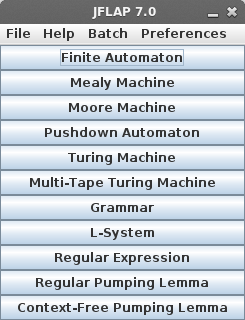
\includegraphics[width=0.23\textwidth]{img/jflap_home.png}
	\end{center}
	\caption{JFLAP home screen.}
	\label{fig:home}
\end{wrapfigure}
\jflap requires \name{JAVA} version 1.6 or higher. You can check the default java version in your system by running the command ``java -version'' in a terminal/console. In case you have an older version of \name{JAVA}, you can get the latest version from \href{http://java.com/en/download/manual.jsp}{here}.

\begin{enumerate}
  \item Please fill out the \href{http://www.cs.duke.edu/csed/jflap/log/form.php}{download form}.
  \item After submitting the form, a page will be shown that has multiple versions to download. Please download the May 15, 2011 version that has SVG included.
  \item \label{cmd:run} Run \jflap with the following command ``java -jar $<$your-download-directory$>$JFLAP.jar''. Replace ``$<$your-download-directory$>$'' token with the actual path of the directory where you downloaded \jflap. You should see the home screen of \jflap (see Figure~\ref{fig:home}).
\end{enumerate}

\jflap is a powerful tool to manipulate various formalisations and all its capabilities can be accessed via its home screen. Do not be alarmed to see options that may not make sense to you at this stage. During the course you will be introduced to these concepts.




\newpage
%%%%%%%%%%%%%%%%%%%%%%%%%%%%%%%%%%%%%%%%%%%%%%%%%%%%%%%%%%%%%%%%%%%%%%%%%%5
\section{Finite Automaton}
%%%%%%%%%%%%%%%%%%%%%%%%%%%%%%%%%%%%%%%%%%%%%%%%%%%%%%%%%%%%%%%%%%%%%%%%%%5

\begin{wrapfigure}{r}{0.4\textwidth}
	\vspace{-20pt}
	\centering
	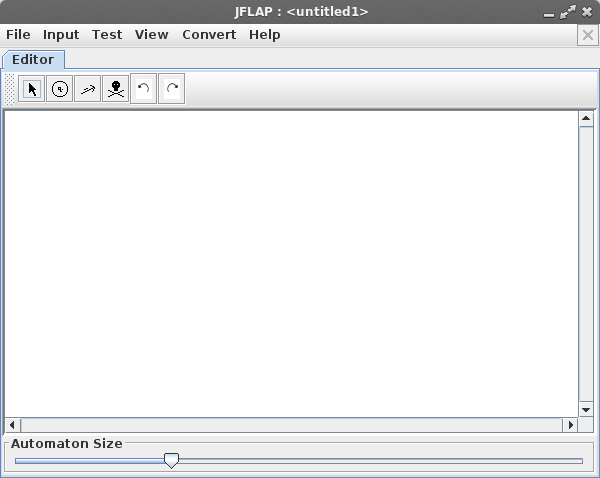
\includegraphics[width=0.4\textwidth]{img/jflap_fa.png}
	\caption{Editor for finite automaton.}
	\label{fig:editor}
\end{wrapfigure}
We will create a simple \emph{finite state automaton} using \jflap. Finite state automatons are simple machines to recognize regular languages. They can be visualized as graphs consisting of states and transitions.
%%
Let us create a simple three state automaton.
%
\begin{enumerate}
  \item Click the ``Finite Automaton'' button (first button from top) on the \jflap home screen.
  \item A new window should be created with an Editor tab opened (see Figure~\ref{fig:editor}).
  \item The image below shows the editor tools seen at the top area of the tab.
  \begin{center}
	   
\includegraphics[width=1\linewidth]{img/fa_tools.png}
  \end{center}
\end{enumerate}

\ 
\subsection{Creating states}

Let us now create and add some states to our FSM:

\begin{center}
		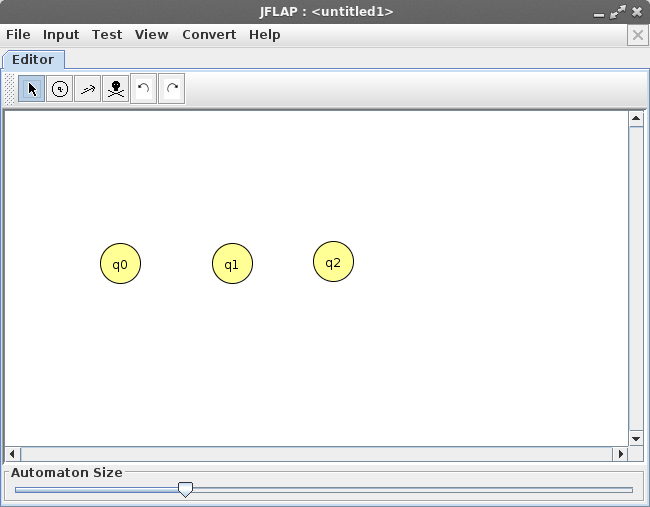
\includegraphics[scale=0.3]{img/fa_states.png}
\end{center}

\begin{enumerate}
  \item Click the create state button and do a left mouse click anywhere in the empty canvas area of the editor. A state with label $q0$ should be created. Do two more left mouse clicks to create states $q1$ and $q2$.
  \item Choose the select tool by doing a left mouse click on the select button in the editor tools.
  \item Right click on the state $q0$. A context menu should appear as shown in the figure below.
  \begin{center}
   \vspace{-0.3cm}\hspace{2em}
   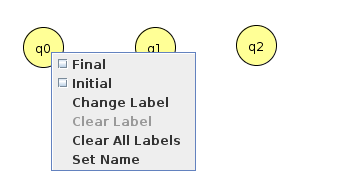
\includegraphics[width=0.4\linewidth]{img/fa_menu.png}
  %\caption{JFLAP Toolset.}
  \label{fig:context}
 \end{center}

 \item Choose ``Initial'' from the menu to make $q0$ as the initial state for the automaton. Similarly, right click on state $q2$ and make it a final state by selecting ``Final''. Observe that $q0$ has a triangle pointing towards it and $q2$ has a double outline.
   \begin{center}
   \vspace{-0.3cm}\hspace{2em}
   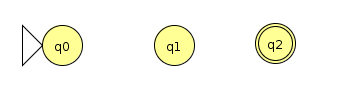
\includegraphics[width=0.4\linewidth]{img/fa_fin.png}
  %\caption{JFLAP Toolset.}
  \label{fig:context}
 \end{center}
\end{enumerate}




\subsection{Creating transitions}

 \begin{enumerate}
   \item Select the create transition tool by doing a left mouse click on it in the editor tools.
   \item Left click and hold on state $q0$ and drag towards state $q1$ without releasing the mouse. Release the mouse once it is over state $q1$. A text input field should appear between the states $q0$ and $q1$ as shown below.
   \begin{center}
  	\vspace{-0.3cm}\hspace{2em}
  	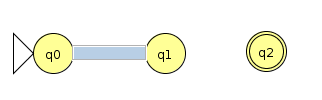
\includegraphics[width=0.27\linewidth]{img/fa_a_input.png}
  	\label{fig:input}
   \end{center}

   \item Type the letter ``$a$'' in the input field and press enter. An arrow with label ``$a$'' should appear between states $q0$ and $q1$. Add another transition between states $q1$ and $q2$ with label ``$b$''. The automaton should now look like the figure below.
   \begin{center}
  	\vspace{-0.3cm}\hspace{2em}
  	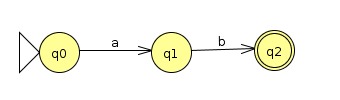
\includegraphics[width=0.28\linewidth]{img/fa_trc.png}
  	\label{fig:input}
   \end{center}

   \item Try deleting the transition between $q1$ and $q2$ using the delete tool and re-creating it again as per the previous step.
   \item In this step we will add a ``loop'' on state $q1$. Select the create transition tool. Left click on state $q1$, drag and release the mouse while in state $q1$. Type the letter ``$c$" in the input text field that appears. You should now see a loop on state $q1$ with label $c$.
   \begin{center}
  \vspace{-0.3cm}\hspace{2em}
  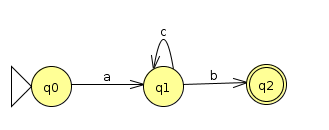
\includegraphics[width=0.28\linewidth]{img/fa_loop.png}
  \label{fig:input}
   \end{center}
 \end{enumerate}

Congratulations! You have just created your first automaton in \jflap.
%



\subsection{Saving and loading files}


Saving and loading files with \jflap is similar to any other software you might have used.
\begin{enumerate}
  \item Select the ``Save as'' sub-menu under the ``File'' menu see on the top of the editor.
  \item Browse to the directory where you want to save the file and enter the file name ``FirstFSA'' before clicking the Save button. \jflap files are saved using the ``jff'' extension.
  \item Exit \jflap.
  \item Open \jflap again (see Step~\ref{cmd:run}  in Section~\ref{sec:downrun}).
  \item From the home screen of \jflap (see Figure~\ref{fig:home}) open the saved file using the File menu.
  \item The Finite Automaton editor should automatically open showing the finite state automaton you just created.
\end{enumerate}



\subsection{Simulations}


Recall that finite state automatons can be used to recognize languages. Let us now test what words can be recognized by the automaton we created. Intuitively, a finite state automaton
\emph{accepts} a word if starting from the initial state the automaton reaches a final state once it has consumed all the symbols in the word.

For example, consider a word $w_1$ consisting of just a single symbol $a$; that is, $w_1=a$.
Our automaton will start from its initial state $q0$, read symbol $a$, and transition to state $q1$. State $q1$ is not an final state and there are no more symbols to read, hence the automaton \emph{terminates} at $q1$ without accepting the word $w_1$.

Consider another word $w_2= ab$. The automaton will begin in its initial state $q0$, read $a$ and transition to $q1$. Once in $q1$ it will read the last remaining symbol $b$ and transition to $q2$. Since $q2$ is a final state and we have read all the input, the automaton terminates in $q2$ accepting the word $w_2$.

Time for some hands-on exercise! Make sure that the automaton we created is open the editor. From the top menu left click Input and select ``Step by State''. A new window will open. Please type the word ``ab'' and press OK.
%
A new tab will open as shown below.


\begin{center}
  \hspace{2em}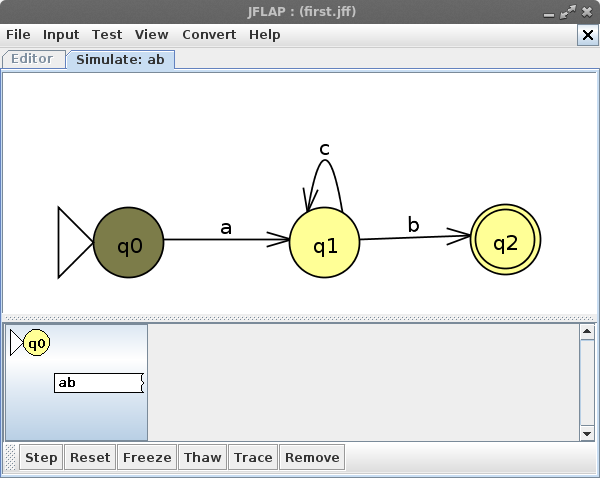
\includegraphics[width=0.5\linewidth]{img/simulate.png}
\end{center}

Press the  ``Step'' button located at the bottom left of the Simulate tab. See how the active state changes as the input is sequentially read. Experiment simulating the automaton with different inputs.
%
Observe the area where the input is mentioned will turn green when an input is accepted and red when an input is rejected.


\end{document} 
%%%%%%%%%%%%%%%%%%%%%%%%%%%%%%%%%%%%%%%%%%%%%%%%%%%%%%
% EOF
%%%%%%%%%%%%%%%%%%%%%%%%%%%%%%%%%%%%%%%%%%%%%%%%%%%%%%
